\documentclass[a4paper,11pt]{book}
\renewcommand{\familydefault}{\sfdefault}

\usepackage{standalone}
\usepackage[english]{babel}
\usepackage[top=3cm]{geometry}
\usepackage{float}
\usepackage{tabularx}
\usepackage{multirow}
\usepackage{booktabs}
\usepackage{pgfplots}
\usepackage{amsmath}
\usepackage{amssymb}
\usepackage{amsfonts}
\usepackage{siunitx}
\usepackage{tikz}
\usepackage{graphics} % for pdf, bitmapped graphics files
\usepackage{graphicx}
\usepackage{exsheets}
\usepackage{algorithm}
\usepackage{algorithmicx}
\usepackage[noend]{algpseudocode}
\usepackage{hyperref}
\usepackage{enumitem}
\usepackage{filecontents}
\usepackage{multirow}
%\usepackage{showframe}% to show frames
%\ifCLASSOPTIONcompsoc
\usepackage[caption=false, font=normalsize, labelfont=sf, textfont=sf]{subfig}
%\else
%\usepackage[caption=false, font=footnotesize]{subfig}
%\fi    

\usetikzlibrary{patterns,arrows,arrows.meta,calc,intersections,shapes,positioning,decorations.pathreplacing,decorations.markings,decorations.pathmorphing}
\usepackage{multicol}

\sisetup{output-decimal-marker={,},exponent-product=\cdot}

\DeclareSIUnit\atm{atm}
\DeclareSIUnit\dioptre{D}



\def\BState{\State\hskip-\ALG@thistlm}


\definecolor{TitleColor}{rgb}{0.65,0.04,0.07}
\definecolor{NumberColor}{rgb}{0.02,0.04,0.48}

\DeclareInstance{exsheets-heading}{fancy}{default}{
toc-reversed = true ,
indent-first = true ,
vscale = 2 ,
pre-code = \IfInsideQuestionT{\rule{\linewidth}{1pt}} ,
post-code =\IfInsideQuestionT{\rule{\linewidth}{1pt}} ,
subtitle-format = \large\scshape\color{rgb:red,0.65;green,0.04;blue,0.07} ,
number-format = \large\bfseries\color{rgb:red,0.02;green,0.04;blue,0.48} ,
points-format = \itshape ,
join = { number[r,B]title[l,B](.333em,0pt);
title[r,B]subtitle[l,B](1em,0pt)
} ,
attach =
{
main[hc,vc]number[hc,vc](0pt,0pt) ;
main[l,vc]subtitle[hc,vc](\marginparsep,0pt)
}
}



\DeclareInstance{exsheets-heading}{block-subtitle}{default}{
vscale = 2 ,
pre-code = \rule{\linewidth}{1pt} ,
post-code = \rule{\linewidth}{1pt} ,%title-format = \large\scshape\color{TitleColor} ,
number-format = \large\bfseries\color{rgb:red,0.02;green,0.04;blue,0.48} ,
subtitle-format = \large\scshape\color{black} ,
join = {
title[r,B]number[l,B](.333em,0pt) ;
title[r,B]subtitle[l,B](1em,0pt)
} ,
attach = {
main[l,vc]title[l,vc](0pt,0pt) ;
main[r,vc]points[l,vc](\marginparsep,0pt)
},
}

\DeclareQuestionClass{textbook}{textbooks}

\SetupExSheets{
  headings = fancy,
  question/print = true ,
  solution/print = false }
 % counter-format = se.qu ,
%  counter-within = section ,
  %question/pre-hook = \rule{\textwidth}{1pt},


\hypersetup{
	colorlinks = true, 
	breaklinks = true, 
	bookmarks = true,
	bookmarksnumbered = true,
	urlcolor = blue, 
	linkcolor = blue, 
	citecolor=blue,
	linktoc=page, 
	pdftitle={}, 
	pdfauthor={\textcopyright Author}, 
	pdfsubject={}, 
	pdfkeywords={}, 
	pdfcreator={pdfLaTeX}, % PDF Creator
	pdfproducer={IEEE} }





\tikzset{point/.style={circle,fill,black!80,inner sep=0pt,minimum size=#1,opacity=0.9}}
\tikzset{point/.default=3pt}\tikzset{vector/.style={line width=1pt,postaction={decorate,decoration={markings,mark=at position 1 with {\arrow{latex}}}}}}
\tikzset{block/.style={rectangle,fill=black!30,draw,minimum size=#1,opacity=0.9,align=center}}
\tikzset{block/.default=15pt}\tikzset{ball/.style={circle,fill=black!30,draw,minimum size=#1,opacity=0.9}}
\tikzset{ball/.default=5pt}\tikzset{pulley/.style={draw=black,line width=0.2pt,circle,minimum size=#1,inner sep=0pt,fill=black!10}}
\tikzset{pulley/.default=20pt}\tikzset{rod/.style={line width=2pt}}
\tikzset{rope/.style={line width=1pt}}
\tikzset{spring/.style={decorate,decoration={coil,amplitude=5pt,segment length=#1,aspect=0.3}}}
\tikzset{spring/.default=5pt}\tikzset{wall/.style={black!10,pattern=north east lines,opacity=0.3}}
\tikzset{ray/.style={line width=0.8pt,postaction={decorate,decoration={markings,mark=at position 0.5 with {\arrow{>}}}}}}
\tikzset{arrow/.style={-latex}}
\tikzset{object/.style={line width=1pt,orange,-latex}}
\tikzset{image/.style={line width=1pt,blue,-latex}}
\tikzset{doublearrow/.style={<->,>=latex,thick}}
\tikzset{brace/.style={decorate,decoration={brace,amplitude=#1}}}
\tikzset{brace/.default=5pt}




\graphicspath{{images/}} 




\makeatletter
\@addtoreset{question}{section}
\makeatother


\begin{document}
\author{Dr. Muhammed Rushdi \and Asem Alaa}

\title{Measurements and Instrumentation [SBE206A] (Fall 2018)\\ Tutorial 3}

\maketitle

\chapter*{Instrument types and performance characteristics (Cont'd)}


\section*{Static characteristics of instruments (Cont'd)}

\begin{itemize}
\item The static characteristics of measuring instruments are concerned only with the steady-state reading that the instrument settles down to, such as accuracy of the reading.
\end{itemize}

\subsection*{Hysteresis}


\begin{figure*}[h!]\label{fig:hysteresis}
\centering
  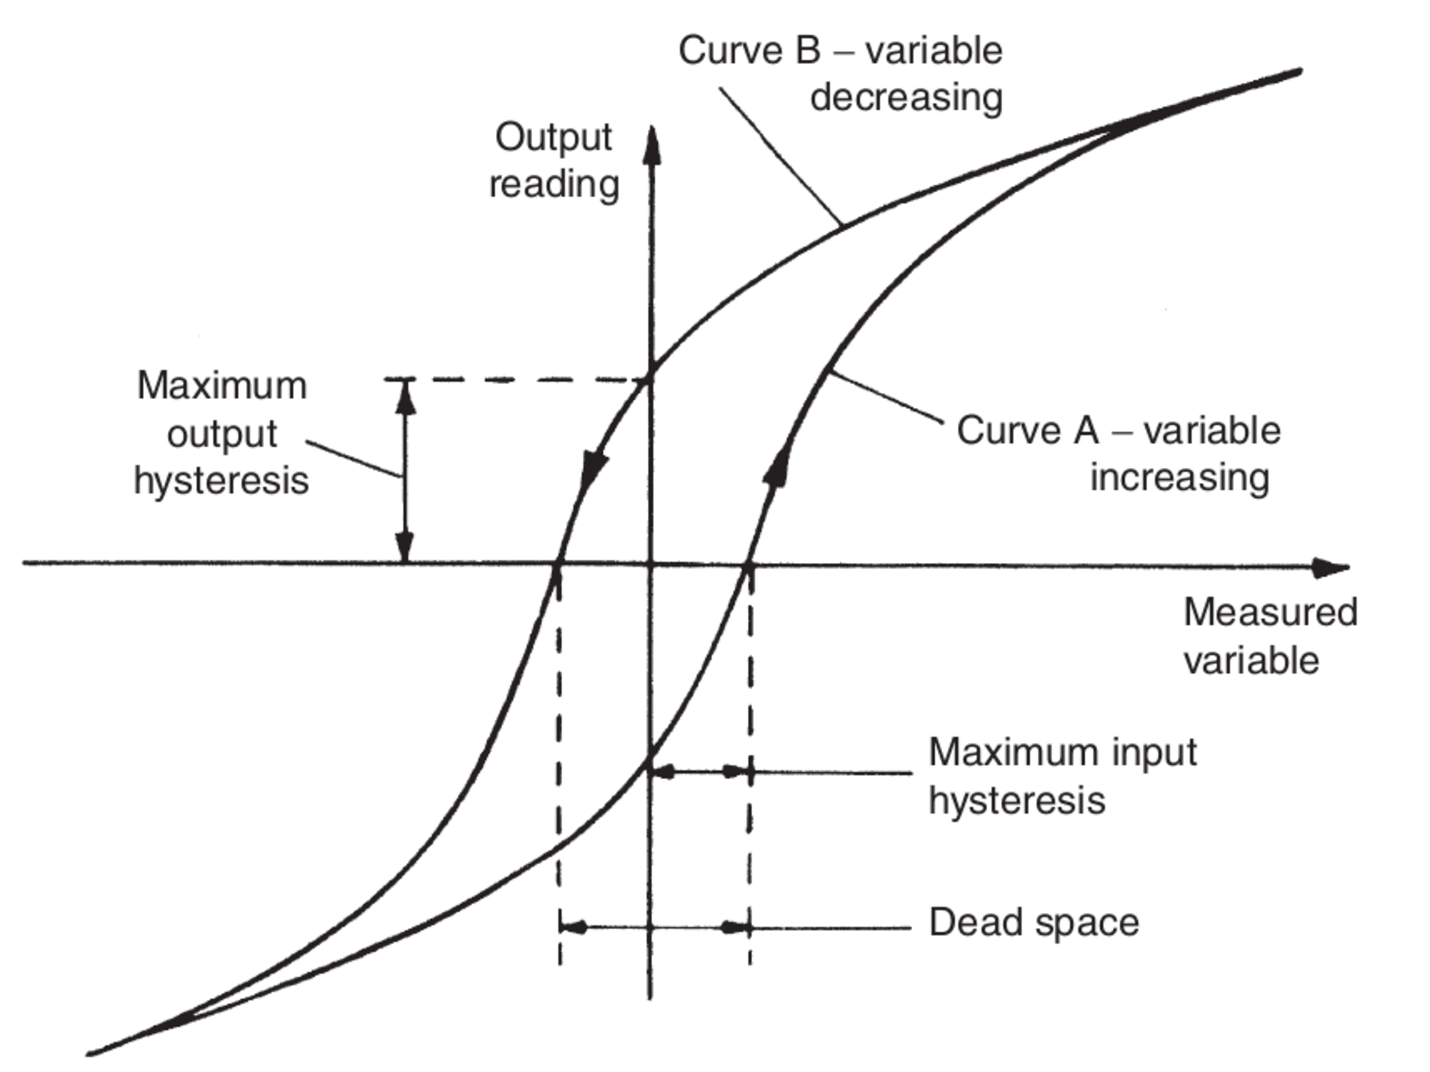
\includegraphics[width=0.7\linewidth]{hysteresis}
  \caption{ Instrument characteristic with hysteresis.} 
\end{figure*}


\subsection*{Dead space}

\begin{figure*}[h!]\label{fig:deadspace}
\centering
  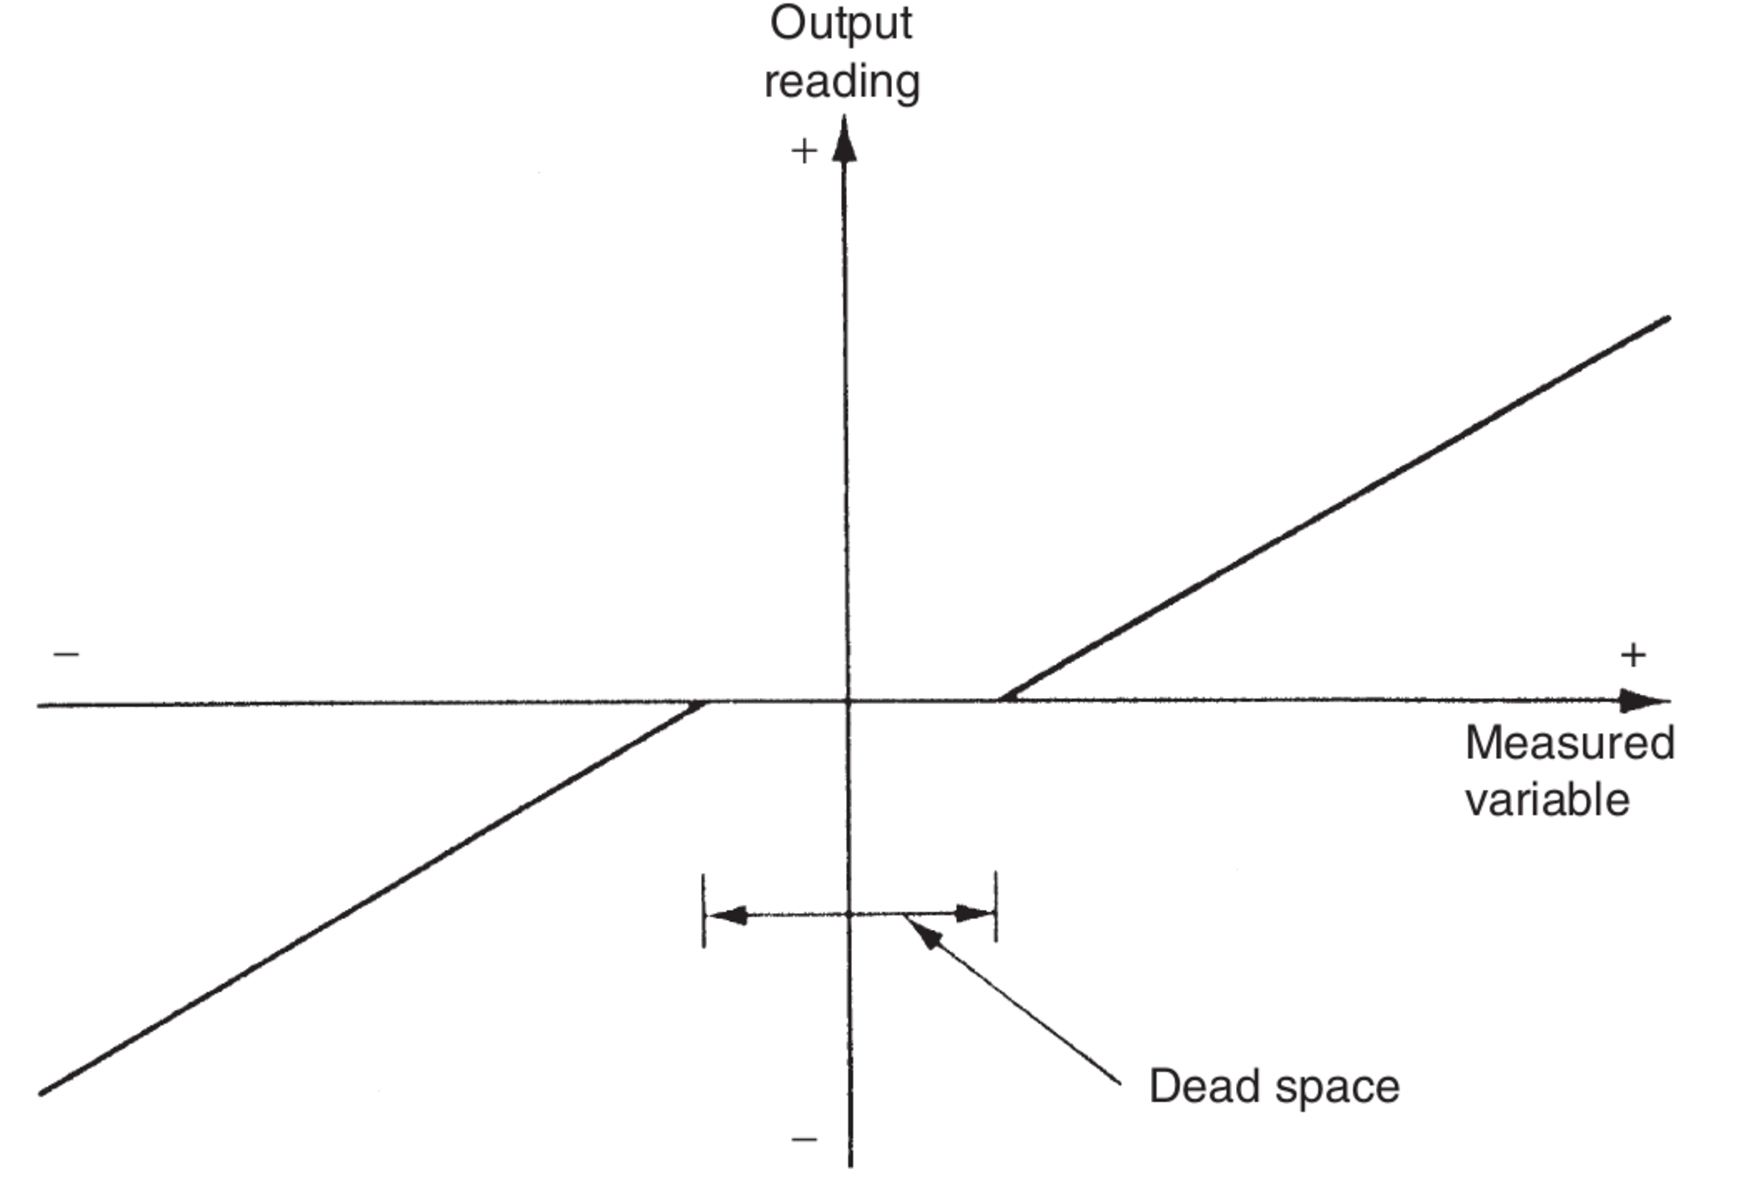
\includegraphics[width=0.7\linewidth]{deadspace}
  \caption{Instrument characteristic with dead space.} 
\end{figure*}

\begin{itemize}
\item Dead space is defined as the range of different input values over which there is no change in
output value.
\item Any instrument that exhibits hysteresis also displays dead space, as marked on Figure \ref{fig:hysteresis}.

\end{itemize}


\section*{Dynamic characteristics of instruments}

\begin{itemize}
\item The dynamic characteristics of a measuring instrument describe its behavior between the time a
measured quantity changes value and the time when the instrument output attains a steady value in
response.
\item In any linear, time-invariant measuring system, the following general relation can be written
between input and output for time $(t)>0$: 
\begin{equation}\label{eqn:dynamic}
a_n \frac{d^{n}q_o}{dt^{n}} + a_{n-1} \frac{d^{n-1}q_o}{dt^{n-1}} + \cdots + a_1 \frac{dq_o}{dt} + a_0 q_o =  b_n \frac{d^{n}q_i}{dt^{n}} + b_{n-1} \frac{d^{n-1}q_i}{dt^{n-1}} + \cdots + b_1 \frac{dq_i}{dt} + b_0 q_i 
\end{equation}
\item If we limit consideration to that of step changes in the measured quantity only, then Equation ~\ref{eqn:dynamic} reduces to:
\begin{equation}\label{eqn:dynamic-reduced}
a_n \frac{d^{n}q_o}{dt^{n}} + a_{n-1} \frac{d^{n-1}q_o}{dt^{n-1}} + \cdots + a_1 \frac{dq_o}{dt} + a_0 q_o =   b_0 q_i 
\end{equation}
\end{itemize}

\subsection*{Zero-order instrument}

\subsection*{First-order instrument}

\subsection*{Second-order instrument}


\begin{question}
A balloon is equipped with temperature and altitude measuring instruments and has radio
equipment that can transmit the output readings of these instruments back to ground. The
balloon is initially anchored to the ground with the instrument output readings in steady state.
The altitude-measuring instrument is approximately zero order and the temperature transducer
first order with a time constant of 15 seconds. The temperature on the ground, $T_0$ , is 10 $^{\circ}$C and the temperature $T_x$  at an altitude of x metres is
given by the relation: \\
$T_x = T_0 − 0.01x$

\begin{enumerate}
\item If the balloon is released at time zero, and thereafter rises upwards at a velocity of 5 metres/second, draw a table showing the temperature and altitude measurements reported
at intervals of 10 seconds over the first 50 seconds of travel. Show also in the table the
error in each temperature reading.
\item  What temperature does the balloon report at an altitude of 5000 metres?
\end{enumerate}

\examspace*{5em}

\end{question}
\begin{solution}


\end{solution}





\begin{question}
Write down the general differential equation describing the dynamic response of a second
order measuring instrument and state the expressions relating the static sensitivity, undamped
natural frequency and damping ratio to the parameters in this differential equation. Sketch
the instrument response for the cases of heavy damping, critical damping and light damping,
and state which of these is the usual target when a second order instrument is being designed.

\examspace*{40em}

\end{question}
\begin{solution}


\end{solution}


\begin{figure*}[h!]\label{fig:comparison}
   
  \subfloat[]{
       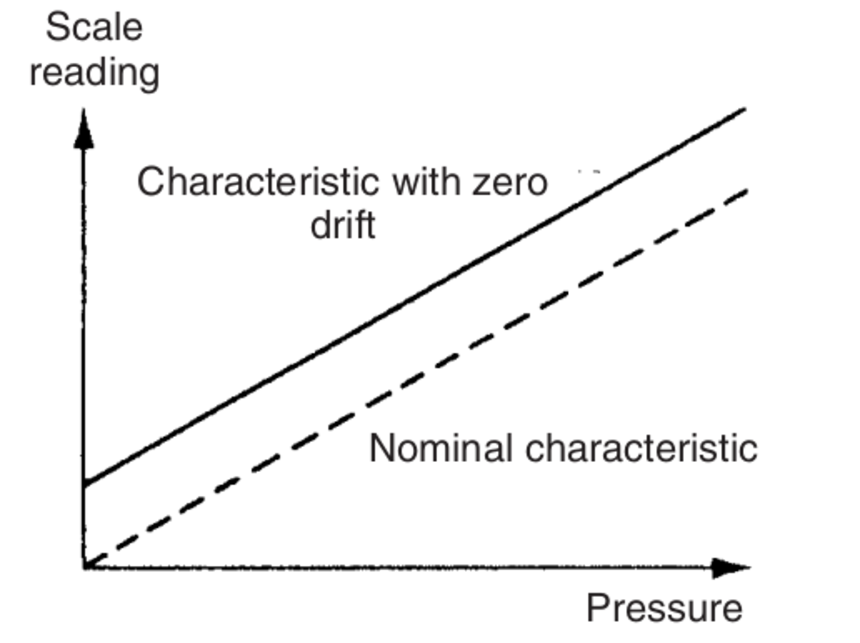
\includegraphics[width=0.40\linewidth]{zdrift}
       }
    \label{fig:zdrift}\hfill
  \subfloat[]{
        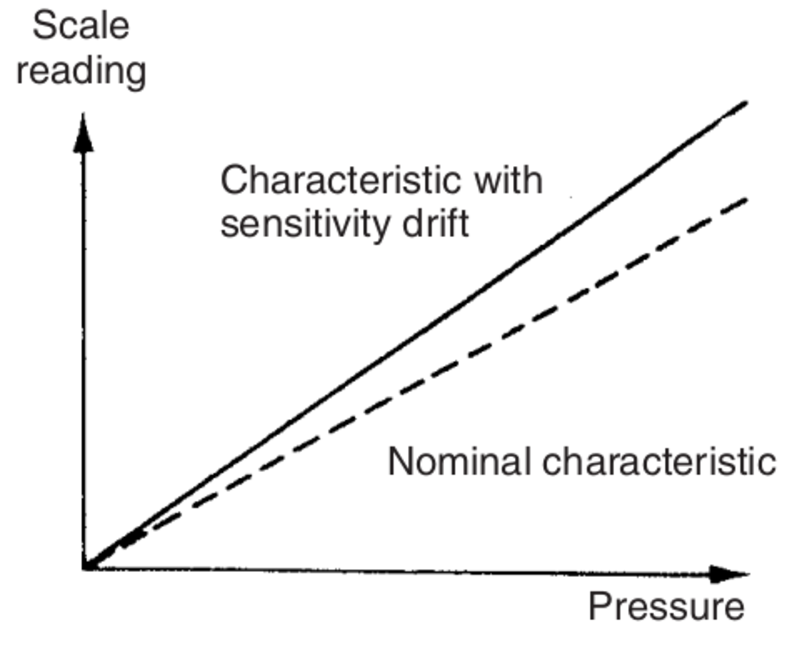
\includegraphics[width=0.40\linewidth]{sdrift}
        }
    \label{fig:sdrift}\\
  \subfloat[]{
       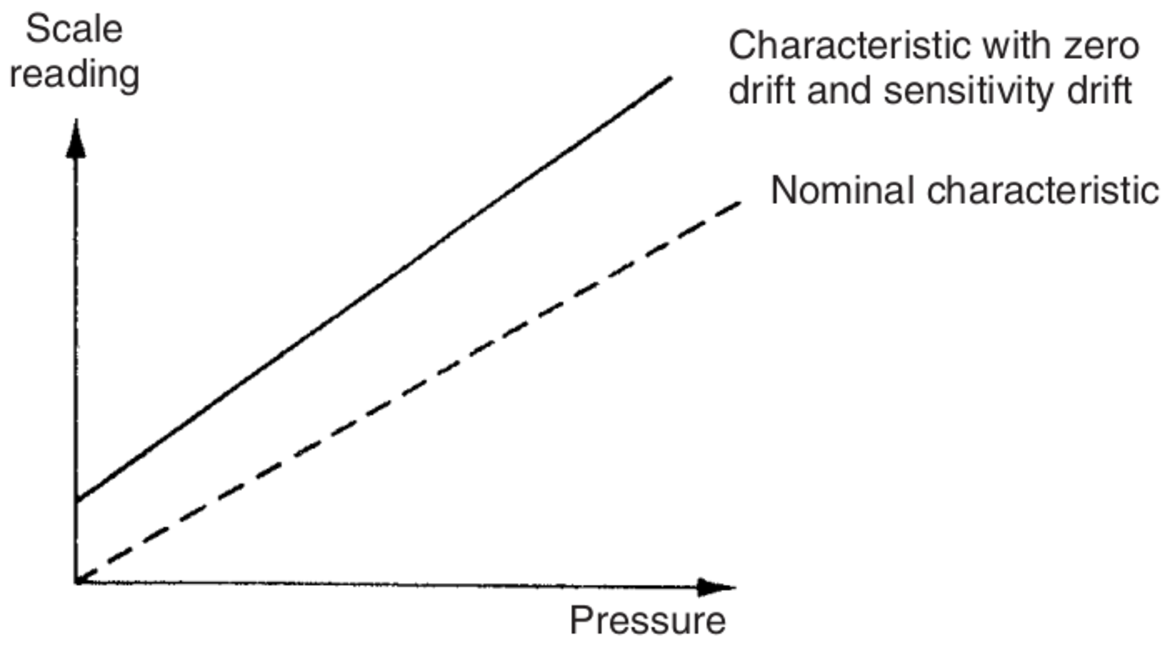
\includegraphics[width=0.40\linewidth]{zsdrift}
        }
   \label{fig:zsdrift}\hfill
  \caption{ Comparison between (a) zero-dirft (b) sensitivity-drift (c) zero- and sensitivity-drift.} 
\end{figure*}

\begin{figure*}[h!]\label{fig:comparison}
  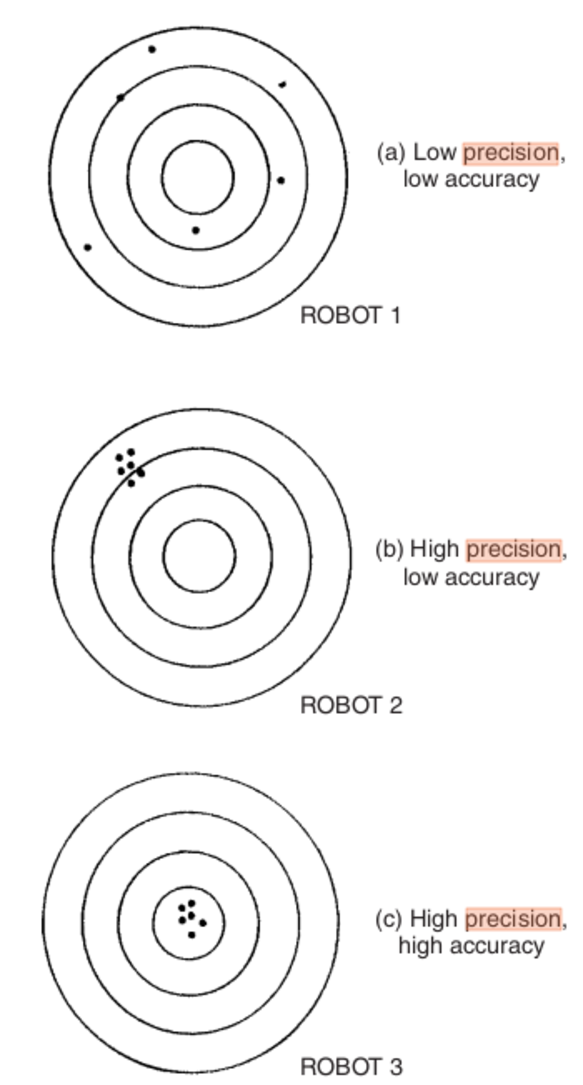
\includegraphics[width=0.40\linewidth]{acc_precision}
  \caption{ Comparison between accuracy and precision.} 
\end{figure*}

\end{document}
